\documentclass[10pt, conference, letterpaper]{IEEEtran}

\usepackage{algorithm}
\usepackage{algorithmicx}
\usepackage{algpseudocode}
\usepackage{amsfonts}
\usepackage{amsmath}
\usepackage{amssymb}
\usepackage[utf8]{inputenc}
\usepackage{xcolor}
\usepackage{mathtools}
\usepackage{graphicx}
\usepackage{caption}
\usepackage{subcaption}
\usepackage{import}
\usepackage{multirow}
\usepackage{cite}
\usepackage[export]{adjustbox}
\usepackage{breqn}
\usepackage{mathrsfs}
\usepackage{acronym}
\usepackage[acronym]{glossaries}
% \usepackage[keeplastbox]{flushend}
\usepackage{setspace}
% \usepackage{stackengine}

\renewcommand{\thetable}{\arabic{table}}
\renewcommand{\thesubtable}{\alph{subtable}}

\DeclareMathOperator*{\argmin}{arg\,min}
\DeclareMathOperator*{\argmax}{arg\,max}

\def\delequal{\mathrel{\ensurestackMath{\stackon[1pt]{=}{\scriptscriptstyle\Delta}}}}

\graphicspath{{./figures/}}
\setlength{\belowcaptionskip}{0mm}
\setlength{\textfloatsep}{8pt}

\newcommand{\eq}[1]{Eq.~\eqref{#1}}
\newcommand{\fig}[1]{Fig.~\ref{#1}}
\newcommand{\tab}[1]{Tab.~\ref{#1}}
\newcommand{\secref}[1]{Section~\ref{#1}}

\newcommand\MR[1]{\textcolor{blue}{#1}}
\newcommand\red[1]{\textcolor{red}{#1}}
\newcommand\DP[1]{\textcolor{green}{#1}}

\newacronym{dsrc}{DSRC}{Dedicated Short Range Communication}
\newacronym{mmWaves}{mmWaves}{millimeter waves}
\newacronym{v2i}{V2I}{Vehicle-to-Infrastructure}
\newacronym{v2v}{V2V}{Vehicle-to-Vehicle}
\newacronym{ue}{UE}{User Equipment}
\newacronym{wave}{WAVE}{Wireless Access in Vehicular Environments}
\newacronym{wimax}{WiMAX}{Worldwide Interoperability for Microwave Access}
\newacronym{los}{LOS}{Line-Of-Sight}
\newacronym{nlos}{NLOS}{Non-Line-Of-Sight}
\newacronym{ber}{BER}{Bit Error Rate}
\newacronym{snr}{SNR}{Signal-to-Noise Ratio}
\newacronym{sinr}{SINR}{Signal-to-Interference-plus-Noise Ratio}
\newacronym{bs}{BS}{Base Station}
\newacronym{ci}{CI}{Confidence Intervals}
\newacronym{gnb}{gNB}{Next Generation Node Bases}
\newacronym{enodeb}{eNodeB}{4G LTE base stations}
\newacronym{nr}{NR}{New Radio}

%\renewcommand{\baselinestretch}{0.98}
% \renewcommand{\bottomfraction}{0.8}
% \setlength{\abovecaptionskip}{0pt}
\setlength{\columnsep}{0.2in}

% \IEEEoverridecommandlockouts\IEEEpubid{\makebox[\columnwidth]{PUT COPYRIGHT NOTICE HERE \hfill} \hspace{\columnsep}\makebox[\columnwidth]{ }} 

\title{Comparison between different technologies for vehicular communication}

\author{Davide Peron$^\dag$
\thanks{$^\dag$Università degli Studi di Padova, email: perondav@dei.unipd.it}
} 

\IEEEoverridecommandlockouts

\begin{document}

\maketitle

\begin{abstract}
Millimeter Wave communication will be a key technology introduced by 5G cellular networks. Thanks to its high frequency, this kind of communication will enable networks with a datarate higher than the one offered by nowadays networks and a very low latency. Unfortunately, due to the high frequency, mmWaves suffer of high sensitivity to blockages and they require antennas with an extremely narrow beam with consequent difficulties in the alignment process.
For this reason, other technologies will support mmWaves to ensure a good reliability also in case of harsh channel conditions at the cost of a lower datarate.

In this work mmWaves are compared with LTE and IEEE 802.11p (DSRC) in order to show the pros and cons of each one, with a view to future applications in which these three technologies can cohexist.
\end{abstract}

\IEEEkeywords
mmWaves, Vehicular Networks, DSRC, LTE, ns3.
\endIEEEkeywords


\input{Intro}

% !TEX root = template.tex

\section{Related Work}
\label{sec:related_work}

Vehicular networks have been studied for years to increase the safety in the streets, to make driving an easier task (with devices like navigators or obstacle sensors) or simply to increase the level of entertainment inside the vehicle.
In the last few years, a lot of companies in the automotive industry tried to install communication modules in their cars to enhance the communication capability with the external environment, the technology that presented the most suitable features has been \gls{dsrc}.
Toyota in \cite{Toyota15} presents some situation in which \gls{v2i} and \gls{v2v} communication would be desirable, their goal is mostly to increase the safety in the streets. In \cite{Cadillac17}, the company introduces \gls{v2v} communication in one of its products to share information with other equipped cars that can be used to alert drivers to upcoming potential hazards. In both these solutions, \gls{dsrc} is used as enabling technology.

The next step in this field will be to exploit the potential of hybrid networking. The motivation for this approach is given by the availability of several communication modules inside the commercial vehicles. Each technology has different characteristics in terms of signal propagation, bandwidth and cost, the goal is to design a system that changes the kind of communication when needed.

Ylianttila et al. \cite{Ylianttila05} propose an algorithm to switch between cellular and Wi-Fi networks. The vehicle's position is updated using GPS signal. Once the vehicle enters the coverage area of a Wi-Fi hotspot, radio signals from the access point are probed and handover towards Wi-Fi network is made only if the received signal's strenght is above a certain threshold.

Wang et al. \cite{Wang16} employ a decision tree to decide when is convenient make handoff towards \gls{wave} and \gls{wimax} from third generation cellular network.
When a vehicle enters in a new access point coverage area, it feeds the decision tree with some predetermined metrics such as network statistics, type of service required or the speed of the vehicle to compute the probability to make handoff.

In \cite{Higuchi17} a novel approach to the problem is proposed, in which interface selection is controlled by a remote central server. The server provides vehicles with recommended interface selection strategies optimized based on statistical knowledge. The vehicles would normally follow server's directives, they can take some controlled decision whenever the actual channel conditions deviates from the statistics on the server.

In this paper we extend the previous work making a comparison between \gls{dsrc}, \gls{mmWaves} and 4G cellular networks in a vehicular scenario, searching for the strenghtness of each technology.

% !TEX root = template.tex

\section{Simulation framework}
\label{sec:simulation_framework}
% The aim of this paper is to compare the behavior of three different communication technologies within a similar scenario. 
To compare different communication technologies, the authors developed three independent scenarios using WAVE, LENA and mmwave module for \textit{ns-3}. The latter is not in the official release but has been developed by University of Padua toghether with New York University (NYU) as an extension of lte module to allow realistic simulations also for higher frequency applications. 

The simulation's scenario is slight different for \gls{dsrc} and the other two technologies. In a realistic scenario, \gls{dsrc} is used mostly in direct \gls{v2v} communication, LTE is more suitable for a \gls{v2i} communication and \gls{mmWaves} can be used both in a \gls{v2v} communication (assuming the vehicles are in line of sight and close to each other and assuming good enough environment conditions) and a \gls{v2i} one.
Nevertheless, in this paper \gls{mmWaves} is considered only for \gls{v2i} communication.

\subsection{DSRC}
\label{sec:dsrc_model}
To simulate the robustness and the feasibility of \gls{dsrc} in our application, two vehicles have been positioned in \gls{los}, they do not move during the simulation and their distance is increased from a minimum of 2 meters to a maximum of 200 meters. This scenario takes into account both the case in which the cars are actually stopped and when, instead, the cars are moving with the same velocity and the same direction.

A vehicle sends to the other 1000 bytes packets using UDP and 3 different inter-packet intervals: $8\mu s$, $80\mu s$ and $0.8s$, that correspond respectively to the datarates: $1Gb/s$, $100Mb/s$ and $10kb/s$.

The simulation has been made using the \gls{wave} module of ns-3 that implements the core features of \gls{dsrc} standards suite \cite{WAVEStandard}.

\subsection{LTE}
LTE is the most used technology in the $4^{th}$ generation cellular networks, therefore is used as backup technology in case \gls{dsrc} or \gls{mmWaves} are not usable due to environment conditions, the requirements of the application to use or any other reason.

The scenario implemented to simulate the behavior of LTE is a square area 500 meters wide in which 6 buildings and \gls{enodeb} (i.e. the LTE base stations in 3GPP \gls{nr} terminology) are randomly positioned.
The number of \gls{enodeb}s positioned in the area increases from 3 to 40. This high density of base stations is irrealistic for LTE, since each \gls{enodeb} can give a coverage up to several km, but is used anyway to have data comparable with \gls{mmWaves}' simulations.
User moves from (100, 490) along x axis with a velocity of $30m/s$ for 10 seconds. During the simulation, it receives 1400 bytes packets from the closest eNodeB at a rate of $1.12 Gb/s$.
An example of a simulated scenario is shown in \fig{fig:scenario}.

Handovers are made from an eNodeB to another if needed to receives in each moment the best signal possible. \textit{LENA} module of ns-3 has been used for the simulation.

\begin{figure}[ht]
\vspace{-0.2in}
  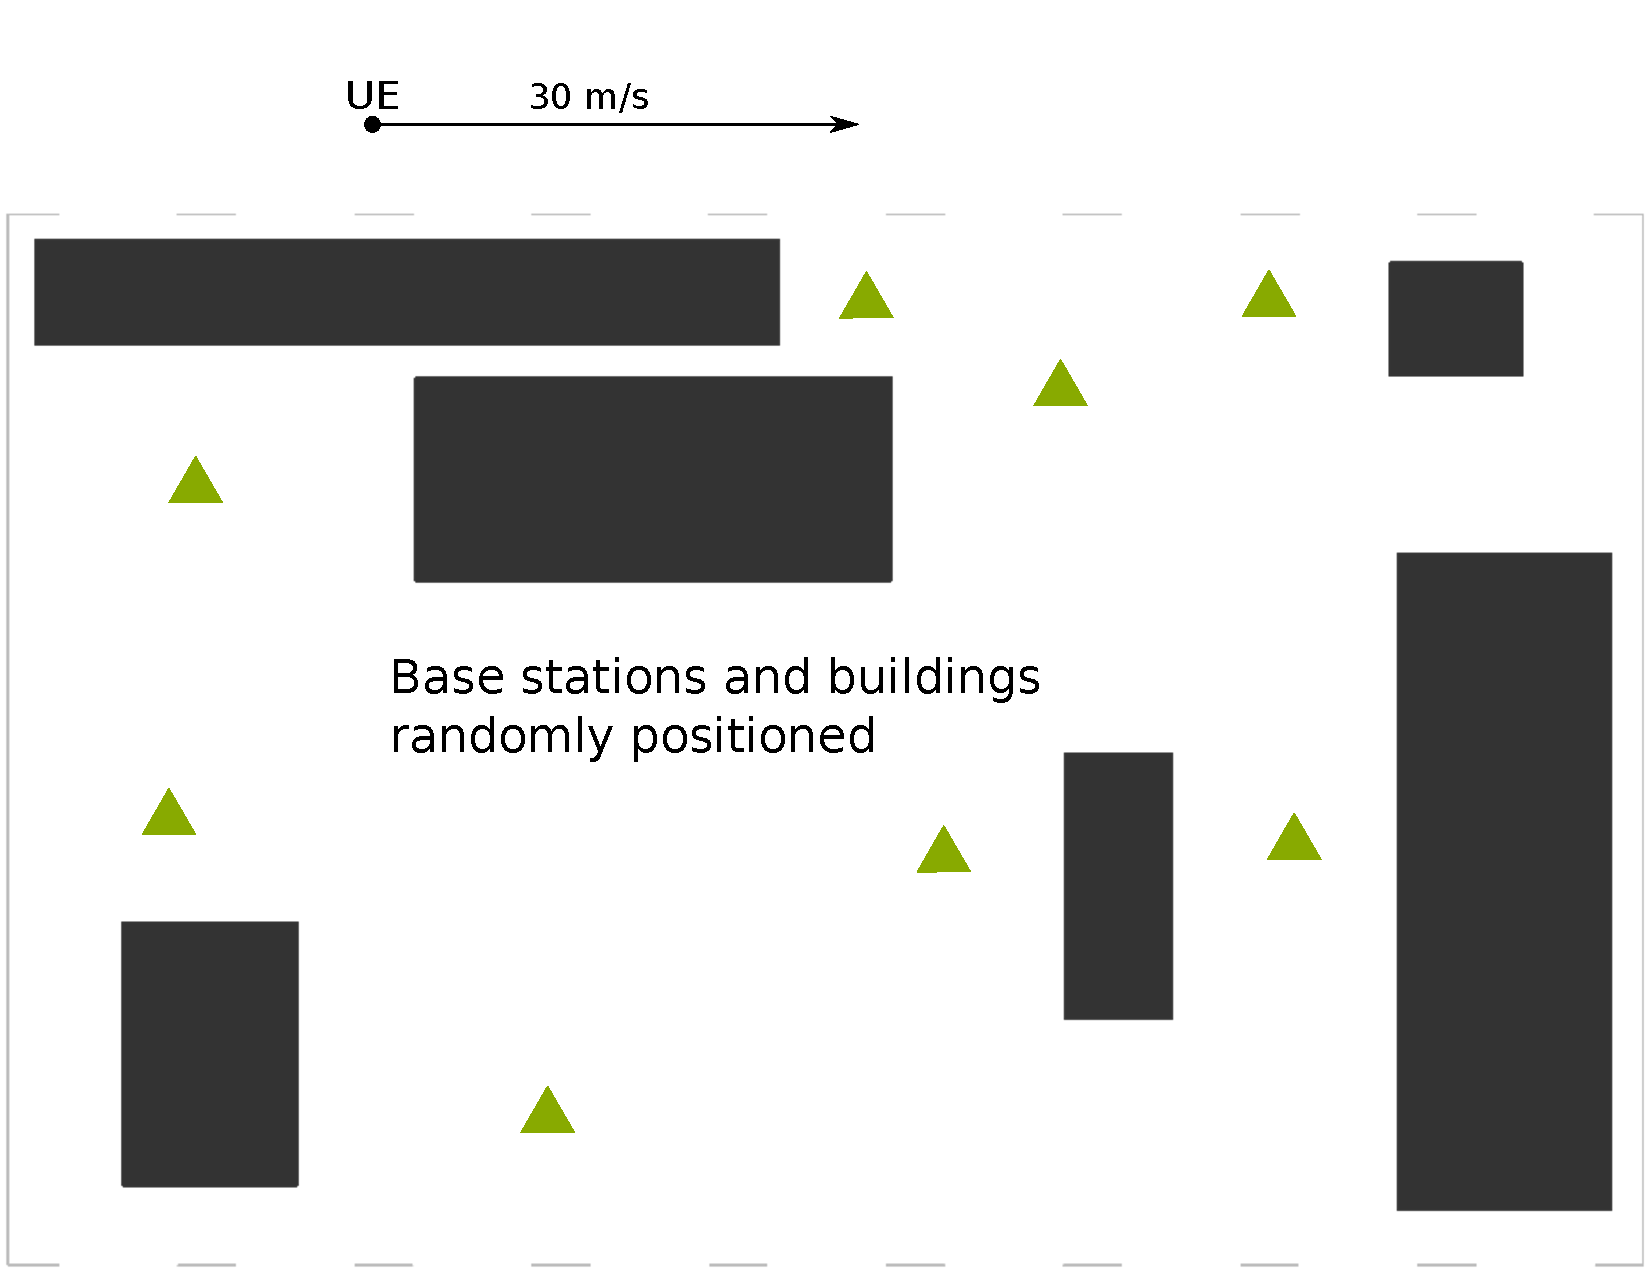
\includegraphics[width=\linewidth]{scenario}
  \caption{Example of a simulation scenario, \gls{enodeb}s and buildings are generated randomly in the designated area.}
  \label{fig:scenario}
\end{figure}

\subsection{mmWaves}
The solution adopted to simulate \gls{mmWaves} is the same used for LTE, this time 40 \gls{gnb} (i.e. the mmWaves base stations in 3GPP \gls{nr} terminology) in a square area 500 meters wide is a realistic scenario since each \gls{gnb} has a very small coverage area due to the blockage problem of high frequency technologies.

For this part, an ns-3 module implemented by University of Padua and NYU has been used \cite{Mezzavilla18}, that implements the PHY and MAC layer of mmWaves in a modular and higly customizable manner.

% !TEX root = template.tex

\section{Results}
\label{sec:results}

\subsection{\gls{dsrc}}


% !TEX root = template.tex

\section{Concluding Remarks}
\label{sec:conclusions}

In this paper, a comparison between \gls{dsrc}, LTE and \gls{mmWaves} has been made, enhanching the pros and cons of each technology.
The conclusions that can be drawn from this work are that each technology is suitable for a set of applications depending on the environment and the datarate.
\gls{dsrc} uses the classic IEEE 802.11 frequency band (5.9 GHz), therefore can be suitable for a dense urban environment, at the cost of a low datarate, since has been found that also data rates such as $100Mb/s$ are too high for this kind of communication.

Having a lower frequency allows also a larger antenna's beam, that makes this technology deployable in a \gls{v2v} scenario.

\gls{mmWaves} can afford very high data rates without losing packets, but it suffers of an high sensitivity to blockages like buildings or even vehicles or people. For this reason is less suitable than \gls{dsrc} for a \gls{v2v} scenario, but is a great choice in a \gls{v2i} one with \gls{bs} in \gls{los}.

The last technology, LTE, is the trade off between \gls{dsrc} and \gls{mmWaves}, since it uses a low enough frequency (less than 10GHz) to be robust to blockages but it can not communicate at the data rates used by \gls{mmWaves}. For this reason is a good backup solution where \gls{mmWaves} \gls{bs} are too far or in \gls{nlos} and a reliable communication is needed.

In the future, more simulations can be made to reduce the \gls{ci} and have more statistically robust results.
The next step on this field is to choose in which context can be used a technology instead of another and how to switch from \gls{mmWaves} to LTE and \gls{dsrc} without losing connection.

\bibliography{biblio}
\bibliographystyle{ieeetr}

\end{document}


